\chapter{Methodology}

\section{Modeling fiber geometry using connection forms}

We utilize the framework described in \cite{de1990ventricular} to describe the geometry of fiber orientation in the heart wall via rotations of a frame field that is fit to the diffusion MRI data. \\
Let a point $\mathbf{x} = \sum_i{x_i\mathbf{e_i}} \in \mathbb{R}^3$ be expressed in terms of $(\mathbf{e_1}, \mathbf{e_2}, \mathbf{e_3})$, the natural basis for $\mathbb{R}^3$. \\
We define a right-handed orthonormal frame field $\mathbf{f_1},\mathbf{f_2},\mathbf{f_3} : \mathbb{R}^3 \to \mathbb{R}^3$. \\ 
Each frame axis can be expressed by the rigid rotation $f_i = \sum_i{a_{i,j}\mathbf{e_j}}$, where $\mathbf{A} = {a_{i,j}} \in \mathbb{R}^{3 \times 3}$ is a differentiable attitude matrix such that $\mathbf{A}^{-1} = \mathbf{A}^T$. \\
Treating $\mathbf{f_i}$ and $\mathbf{e_j}$ as symbols, we can write:
\begin{equation}
\begin{bmatrix}
    \mathbf{f_1} \\
    \mathbf{f_2} \\
    \mathbf{f_3}
\end{bmatrix} = \mathbf{A} \times \begin{bmatrix}
    \mathbf{e_1} \\
    \mathbf{e_2} \\
    \mathbf{e_3}
\end{bmatrix}
\end{equation}

Since each $\mathbf{e_i}$ is constant, the differential geometry of the frame field is completely characterized by $\mathbf{A}$. Taking the exterior derivative on both sides, we have:
\begin{equation} \label{eq:1}
\begin{split}
    \partial \begin{bmatrix}
                \mathbf{f_1} \\
                \mathbf{f_2} \\
                \mathbf{f_3}
            \end{bmatrix} &= (\partial \mathbf{A})\mathbf{A}^{-1}  \begin{bmatrix}
                \mathbf{f_1} \\
                \mathbf{f_2} \\
                \mathbf{f_3}
            \end{bmatrix} \\
            &= \mathbf{C}
            \begin{bmatrix}
                \mathbf{f_1} \\
                \mathbf{f_2} \\
                \mathbf{f_3}
            \end{bmatrix}
\end{split}
\end{equation}
where $\partial$ denotes the exterior derivative, and $\mathbf{C} = (\partial \mathbf{A}) \mathbf{A}^{-1} = (c_{i,j}) \in \mathbb{R}^{3 \times 3}$ is the Maurer-Cartan matrix of connection forms $(c_{i,j})$. \\
Writing $\mathbf{f}_i$ as symbols, \ref{eq:1} is to be understood as $\partial \mathbf{f}_i = \sum_j{c_{i,j}\mathbf{f}_j}$. \\
The Maurer-Cartan matrix is skew symmetric with zeros as diagonal entries so there are at most 3 independent, non-zero 1-forms: $c_{1,2}$, $c_{1,3}$, and $c_{2,3}$. \\
1-forms operate on tangent vectors through contraction, written as $\partial \omega \langle \boldsymbol{\upsilon} \rangle \in \mathbb{R}$ for a general 1-form $\partial \omega = \sum_i{\omega_i \mathbf{e_i}}$ and tangent vector $\boldsymbol{\upsilon} \in \mathbb{R}^3$, which yields:
\begin{equation}
\begin{split}
    \partial \omega \langle \boldsymbol{\upsilon} \rangle &= \sum_i{\omega_i \partial \mathbf{e_i}} \big{\langle} \sum_j{\upsilon_j \mathbf{e_j}} \big{\rangle} \\
    &= \sum_i{\omega_i \upsilon_i}
\end{split}
\end{equation} since $\partial \mathbf{e_i} \langle \mathbf{e_j} \rangle = \delta_{i,j}$, where $\delta_{i,j}$ is the Kronecker delta. \\
It turns out that the space of linear models for smoothly varying frame fields is parametrized by the 1-forms $c_{i,j}$. Since only 3 unique non-zero combinations of $c_{i,j}$ are possible, there are in total 9 connections $c_{i,j,k}$. These coefficients express the rate of turn of the frame vector $\mathbf{f}_i$ towards $\mathbf{f}_j$ when $\mathbf{x}$ moves in the direction $\mathbf{f}_k$. With $\mathbf{f}_1$ taken as the local orientation of a fiber and $\mathbf{f}_3$ taken to be the component of the heart wall normal orthogonal to $\mathbf{f}_1$, \ref{fig:c123theory} illustrates the connection $c_{1,2,3}$, which measures the rotation of fibers for a transmural penetration of the wall. The histograms of $c_{1,2,3}$ for these cases are discussed in Section ???. \\
\begin{figure}[h!]
    \centering
    \begin{subfigure}[h!]{0.3\textwidth}
        \centering
        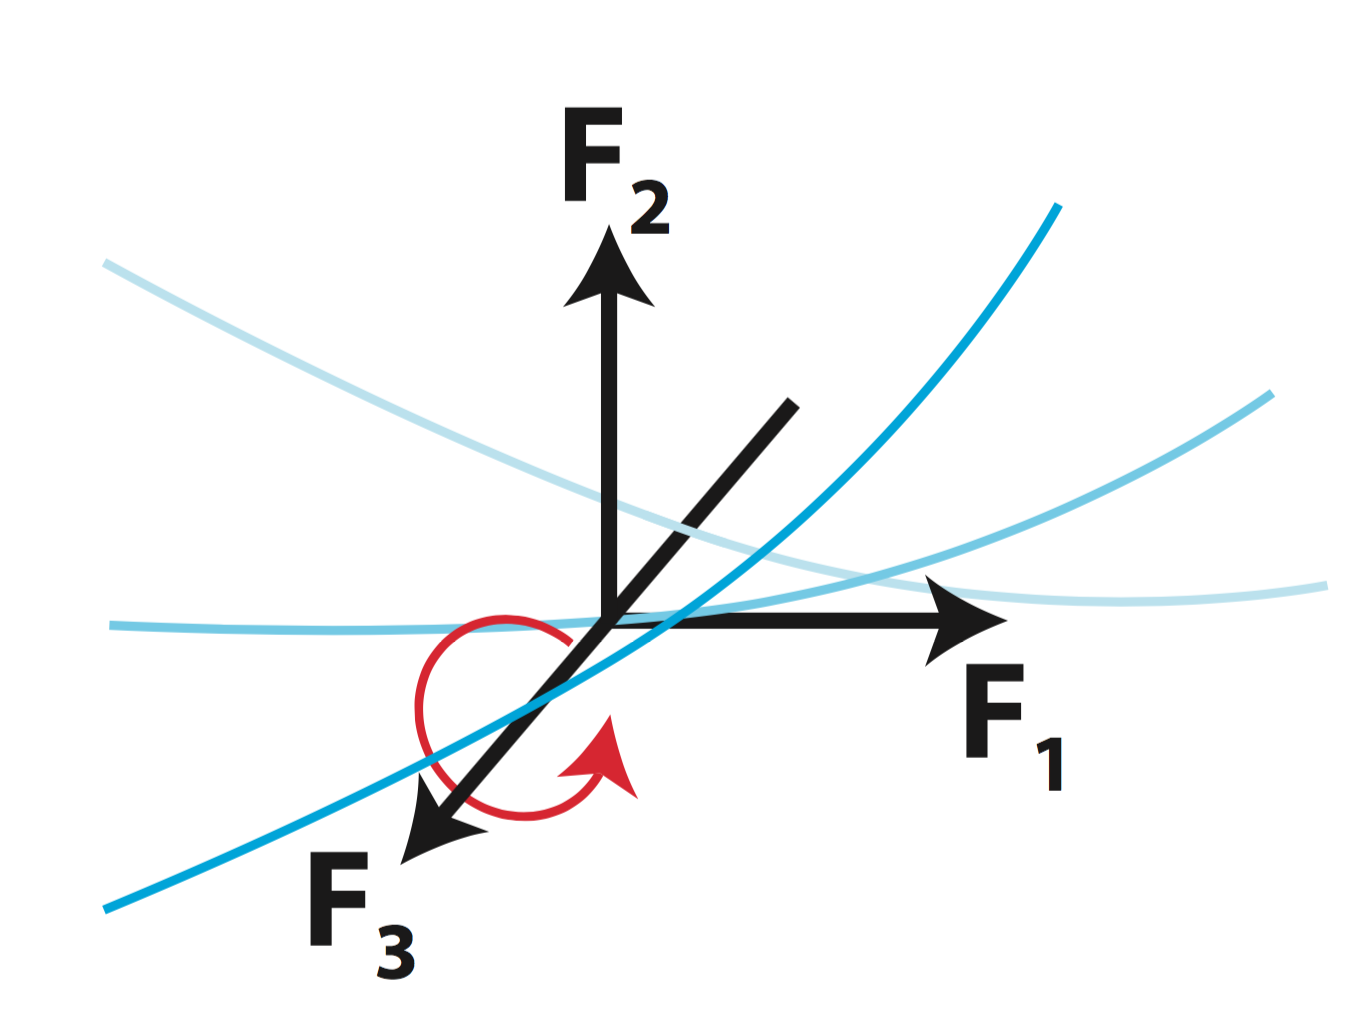
\includegraphics[width=\textwidth]{figures/c123}
        \caption{$c_{1,2,3}$}
        \label{fig:c123theory}
    \end{subfigure}
    \hfill
    \begin{subfigure}[h!]{0.3\textwidth}
        \centering
        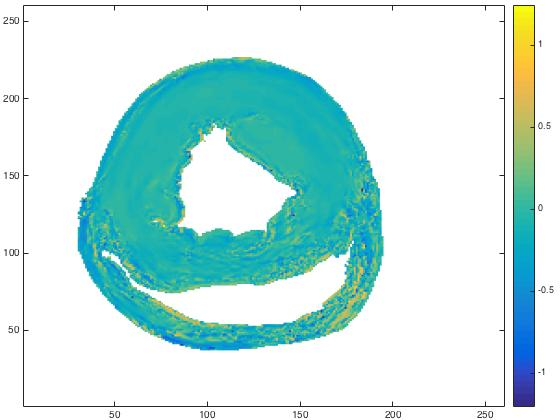
\includegraphics[width=\textwidth]{figures/pig4_c123_slice_19}
        \caption{$c_{1,2,3}$ (infarcted)}
        \label{fig:c123infarcted}
    \end{subfigure}
    \hfill
    \begin{subfigure}[h!]{0.3\textwidth}
        \centering
        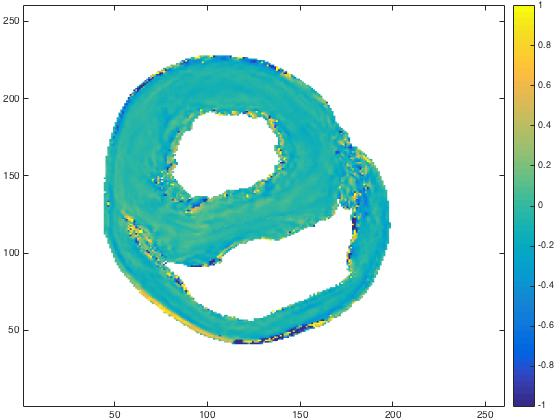
\includegraphics[width=\textwidth]{figures/pig25_c123_slice_30}
        \caption{$c_{1,2,3}$ (healthy)}
        \label{fig:c123healthy}
    \end{subfigure}
    \caption{$c_{1,2,3}$ with range of values in porcine hearts}
    \label{fig:c123}
\end{figure}

 Connection forms measure the local rotations of the frame axes $\mathbf{f}_1, \mathbf{f}_2, \mathbf{f}_3$. Here we focus on the contraction of the 1-form $c_{1,2}$ on the frame axes $\mathbf{f}_3$ and compare its values in a short axis slice of a pig heart with an infarct \ref{fig:c123infarct} with those in a short axis slice from a healthy pig heart \ref{fig:c123healthy}. \\
 
 \begin{figure}
     \centering
     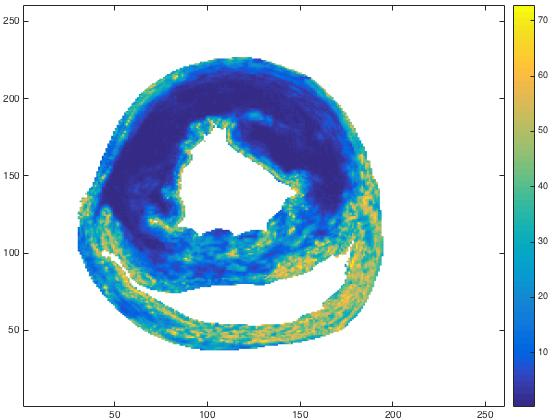
\includegraphics[width=\textwidth]{figures/pig4_error_of_fit_slice_19}
     \caption{Error of fit}
     \label{fig:error_of_fit}
 \end{figure}
 
Cartan frame field analysis applies to smoothly rotating frame fields. In the presence of infarcts fiber orientation coherence is lost. The connections then fail to explain the orientation of fibers in a local neighborhood and fitting errors using this method go up \ref{fig:error_of_fit}. This association of frame field fitting error with fiber incoherence is the key insight behind the developments in this paper.

\section{Cartan Frame Fitting and Error Analysis}

As explained earlier, at each voxel we use an estimate of the fiber orientation given by the orientation of the first principal eigen vector of a diffusion tensor reconstruction for $\mathbf{f}_1$. We then estimate the heart wall normal as the gradient of the distance function to the boundary of the myocardium and take the component of the normal that is orthogonal to $\mathbf{f}_1$ to be $\mathbf{f}_3$. $\mathbf{f}_2$ is then taken to be their cross product. Our numerical implementation of frame field fitting relies on finding the best estimates of the 9 connections at each voxel in the sense of explaining the orientations in its neighborhood. Specifically, using Nelder-Mead optimization, we minimize an energy given by the angle between the measured orientation at each neighbor and that given by rotating the frame field by a particular set of connections. Once this method converges the error of fit at a voxel is taken to be the average angular error between fiber orientations in a neighborhood and those given by rotating the frame at that voxel using its connection parameters.